\section{Results}
\label{sec:results}

\subsection{Self-Critique Induces Larger Representational Drift}

\Figref{fig:cosine} shows the per-layer cosine similarity between base activations and each condition. Across all layers beyond the embedding, critique activations consistently show lower cosine similarity to base than paraphrase activations (mean 0.905 vs.\ 0.946). The difference is statistically significant in 29 of 33 layers after Bonferroni correction, with only the embedding and first three transformer blocks failing to reach significance.

\begin{figure}[t]
    \centering
    \begin{subfigure}[b]{0.48\textwidth}
        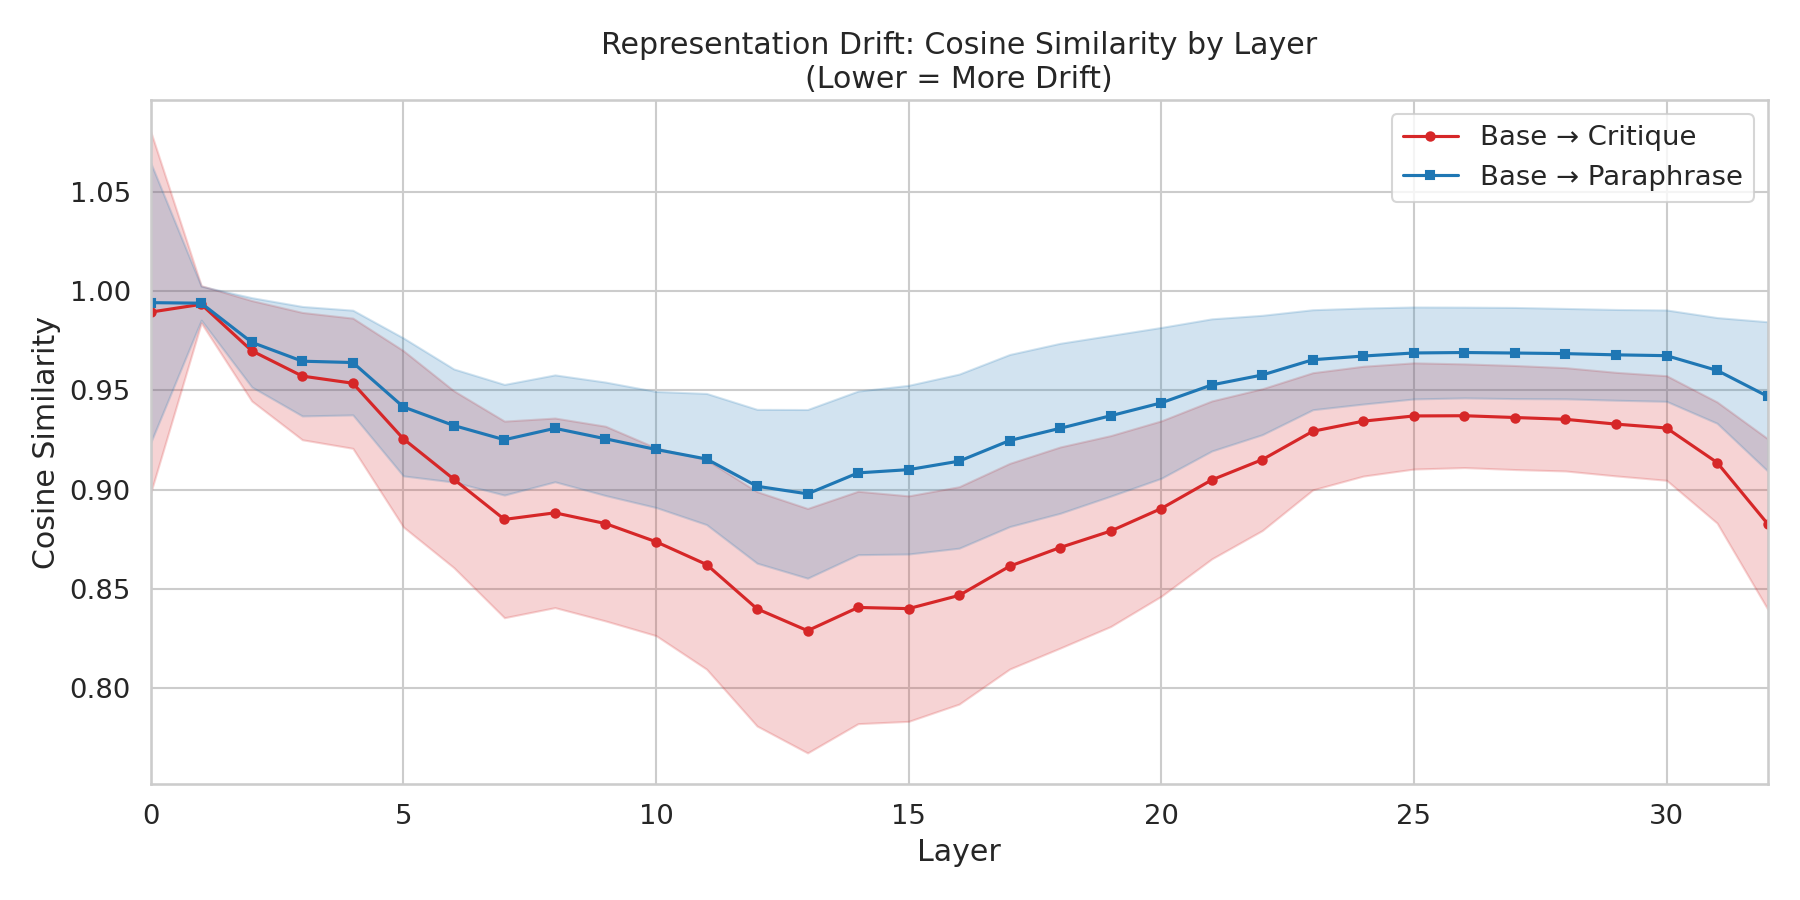
\includegraphics[width=\textwidth]{figures/cosine_similarity_per_layer.png}
        \caption{Cosine similarity}
        \label{fig:cosine}
    \end{subfigure}
    \hfill
    \begin{subfigure}[b]{0.48\textwidth}
        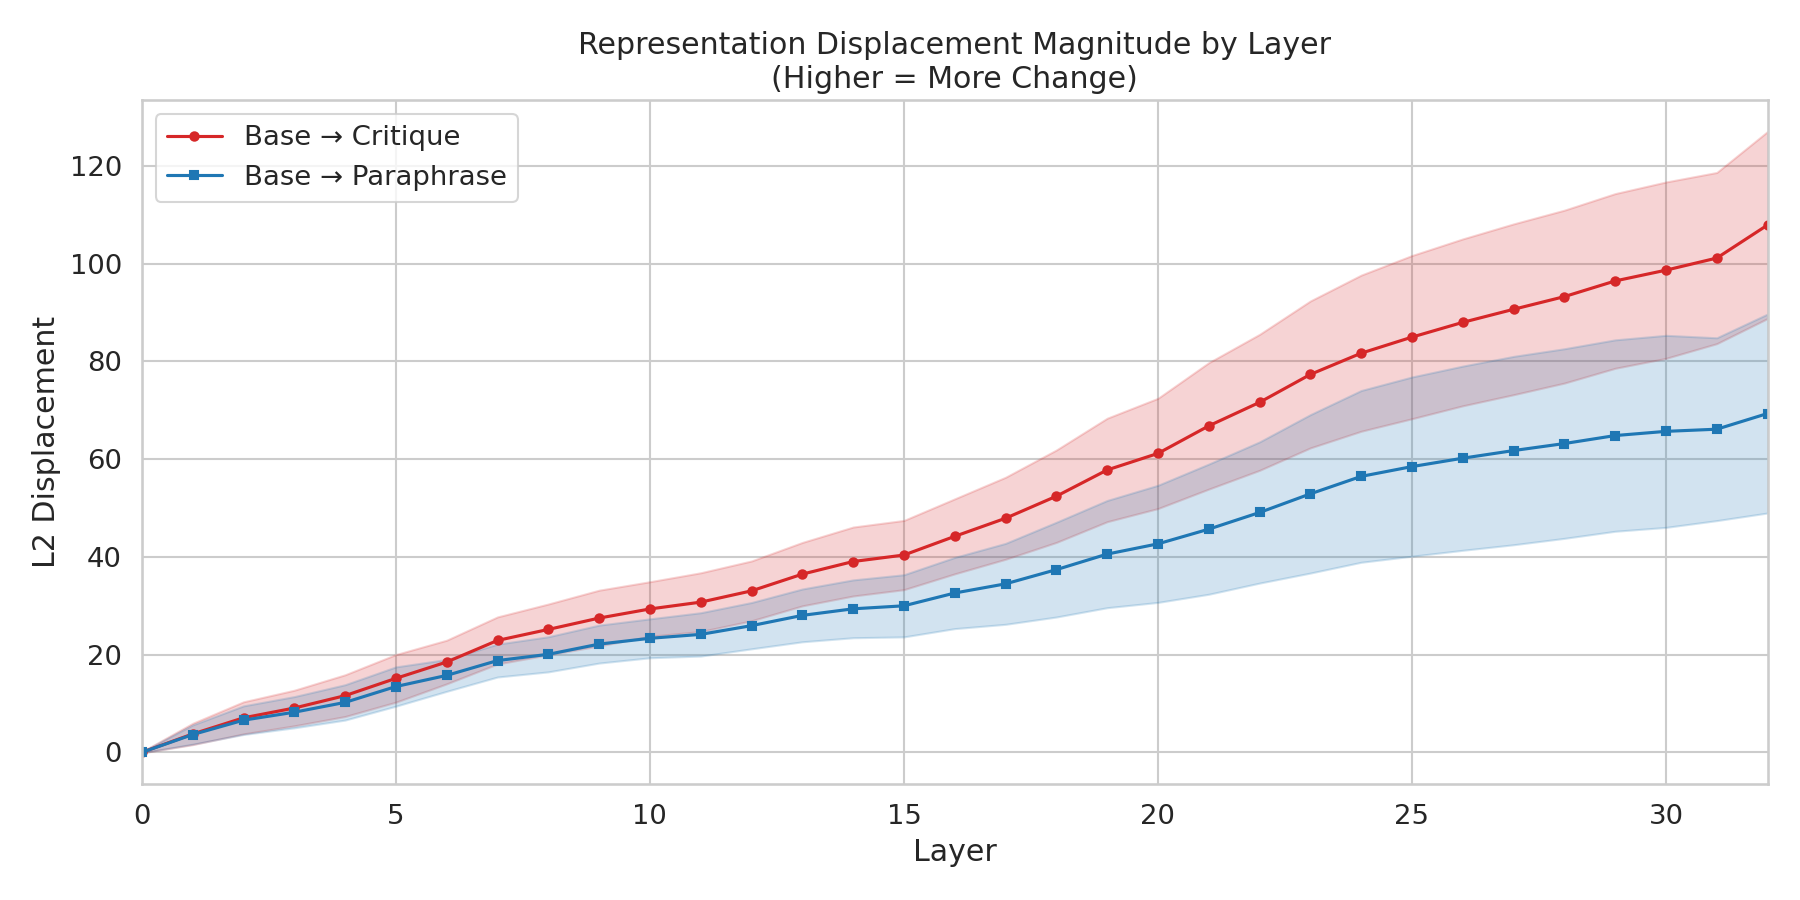
\includegraphics[width=\textwidth]{figures/displacement_per_layer.png}
        \caption{$L_2$ displacement}
        \label{fig:displacement}
    \end{subfigure}
    \caption{Per-layer comparison of representational drift between critique and paraphrase conditions, measured relative to base activations. \captiona Cosine similarity (lower = more drift). \captionb $L_2$ displacement (higher = more drift). Critique induces consistently larger drift across all layers, with the gap widening in middle layers (12--16).}
    \label{fig:drift}
\end{figure}

\Tabref{tab:cosine} presents cosine similarity at selected layers. The largest gap between conditions occurs at layers 12--16 (difference of 0.062--0.068), corresponding to approximately 40--50\% of network depth. $L_2$ displacement tells the same story: critique produces 41\% larger average displacement than paraphrase (50.7 vs.\ 35.8; \figref{fig:displacement}).

\begin{table}[t]
    \centering
    \caption{Cosine similarity between base and condition activations at selected layers. Lower values indicate greater drift. The difference column shows the gap between conditions. Best (largest) differences in \textbf{bold}.}
    \begin{tabular}{@{}lccc@{}}
        \toprule
        Layer & Base$\to$Critique & Base$\to$Paraphrase & Difference \\
        \midrule
        0 (embed) & 0.990 & 0.994 & 0.005 \\
        8 & 0.888 & 0.931 & 0.043 \\
        12 & 0.840 & 0.902 & 0.062 \\
        16 & 0.847 & 0.914 & \textbf{0.068} \\
        24 & 0.935 & 0.967 & 0.033 \\
        32 & 0.883 & 0.947 & 0.064 \\
        \midrule
        Average & 0.905 & 0.946 & 0.041 \\
        \bottomrule
    \end{tabular}
    \label{tab:cosine}
\end{table}

\subsection{Drift Is Concentrated in Middle Layers}

The cosine similarity gap between critique and paraphrase peaks at layers 12--16 (\tabref{tab:cosine}), with layer 16 showing the largest difference (0.068). This concentration at approximately 40--50\% of network depth aligns with findings from \citet{polo2026emergent}, who report that middle layers initiate geometric restructuring during reasoning. \Figref{fig:pvalues} shows that $p$-values drop below $10^{-14}$ from layer 8 onward, indicating robust statistical significance throughout the deeper layers.

\begin{figure}[t]
    \centering
    \begin{subfigure}[b]{0.48\textwidth}
        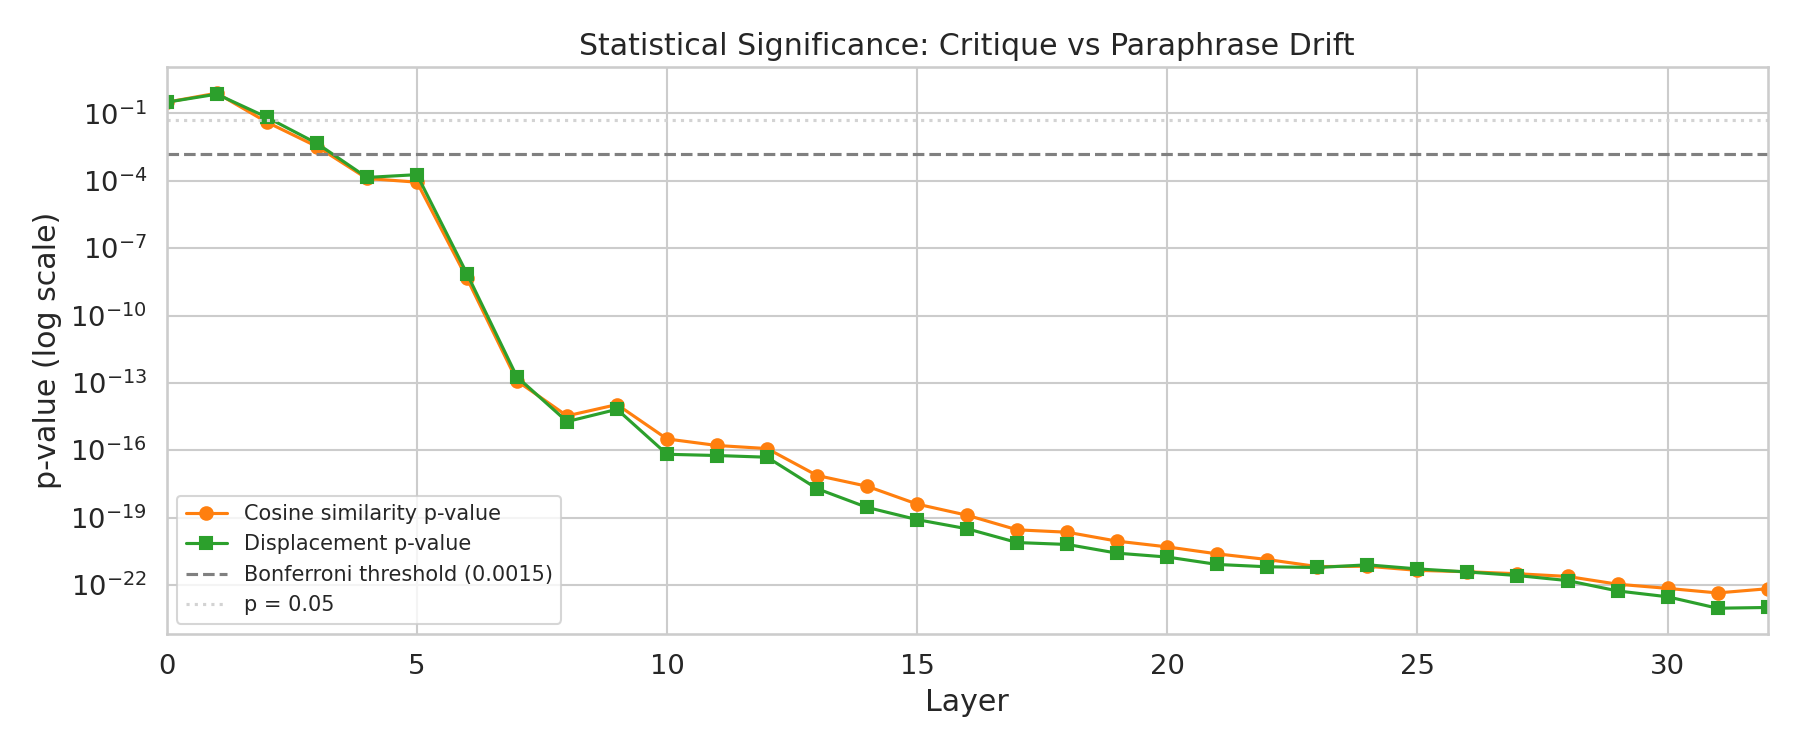
\includegraphics[width=\textwidth]{figures/pvalues_per_layer.png}
        \caption{$p$-values (log scale)}
        \label{fig:pvalues}
    \end{subfigure}
    \hfill
    \begin{subfigure}[b]{0.48\textwidth}
        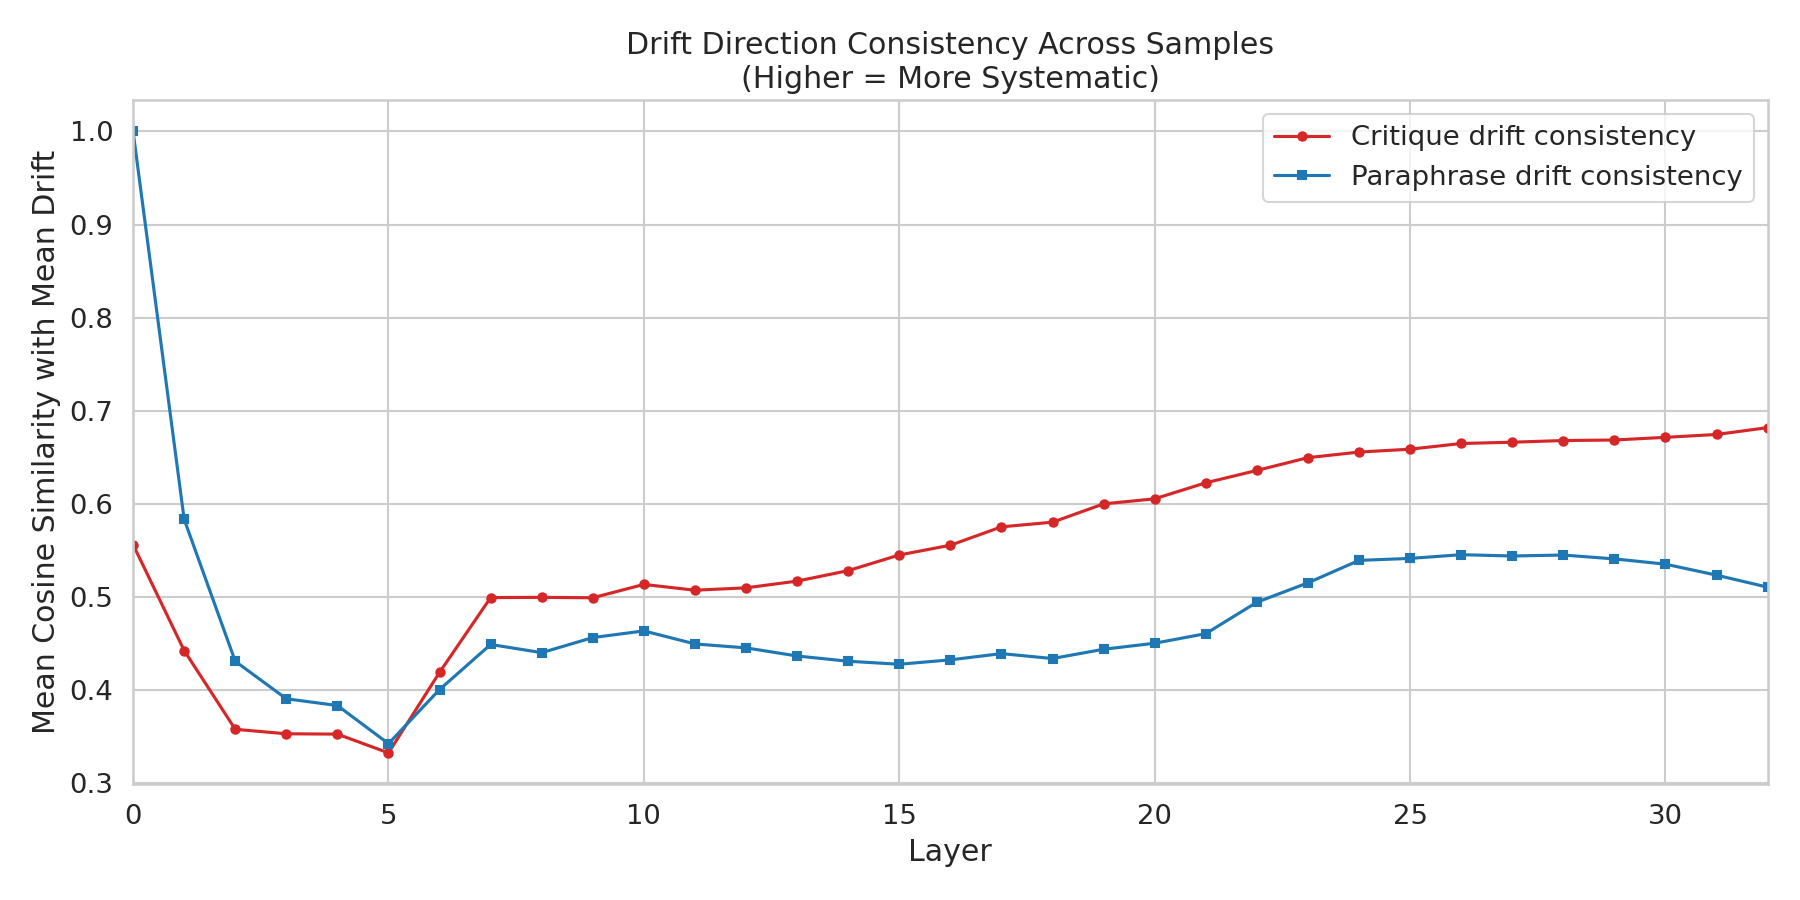
\includegraphics[width=\textwidth]{figures/drift_consistency.png}
        \caption{Drift direction consistency}
        \label{fig:consistency}
    \end{subfigure}
    \caption{\captiona Statistical significance of the difference in cosine similarity between critique and paraphrase conditions (Wilcoxon signed-rank test). The dashed line indicates the Bonferroni-corrected threshold ($\alpha/33$). Layers 4--32 are all significant. \captionb Cosine consistency of drift vectors with their mean direction. Critique drift becomes more consistent than paraphrase drift from layer 7 onward.}
    \label{fig:stats}
\end{figure}

\subsection{Critique Drift Is Directionally Consistent}

We measure whether drift vectors point in a consistent direction across samples. \Figref{fig:consistency} shows that in layers 10--30, critique drift vectors have higher average cosine similarity with their mean direction (0.596) than paraphrase drift vectors (0.479). This indicates that critique induces a systematic directional shift---a ``critique subspace''---rather than random perturbation.

An interesting pattern emerges in early layers: critique drift starts \emph{less} consistent than paraphrase in layers 0--5 but becomes \emph{more} consistent from layer 7 onward. This suggests that self-critique processing is initially noisy but converges to a systematic direction as deeper layers extract the evaluative signal.

\subsection{CKA Confirms Population-Level Restructuring}

\begin{table}[t]
    \centering
    \caption{Average Centered Kernel Alignment (CKA) between conditions across all layers. Lower values indicate more divergent representational structure. Critique creates substantially different structure from both base and paraphrase conditions.}
    \begin{tabular}{@{}lc@{}}
        \toprule
        Comparison & Average CKA \\
        \midrule
        Base $\leftrightarrow$ Paraphrase & 0.428 \\
        Base $\leftrightarrow$ Critique & \textbf{0.224} \\
        Critique $\leftrightarrow$ Paraphrase & 0.236 \\
        \bottomrule
    \end{tabular}
    \label{tab:cka}
\end{table}

\Tabref{tab:cka} shows that base$\leftrightarrow$critique CKA (0.224) is roughly half of base$\leftrightarrow$paraphrase CKA (0.428). This indicates that critique does not merely shift individual activations but reorganizes the population-level covariance structure. \Figref{fig:cka} reveals a non-monotonic pattern: base$\leftrightarrow$paraphrase CKA peaks around layers 12--14 before declining, suggesting that mid-layer representations capture semantic content (preserved in paraphrase) while later layers encode task-specific features (disrupted by critique).

\begin{figure}[t]
    \centering
    \begin{subfigure}[b]{0.48\textwidth}
        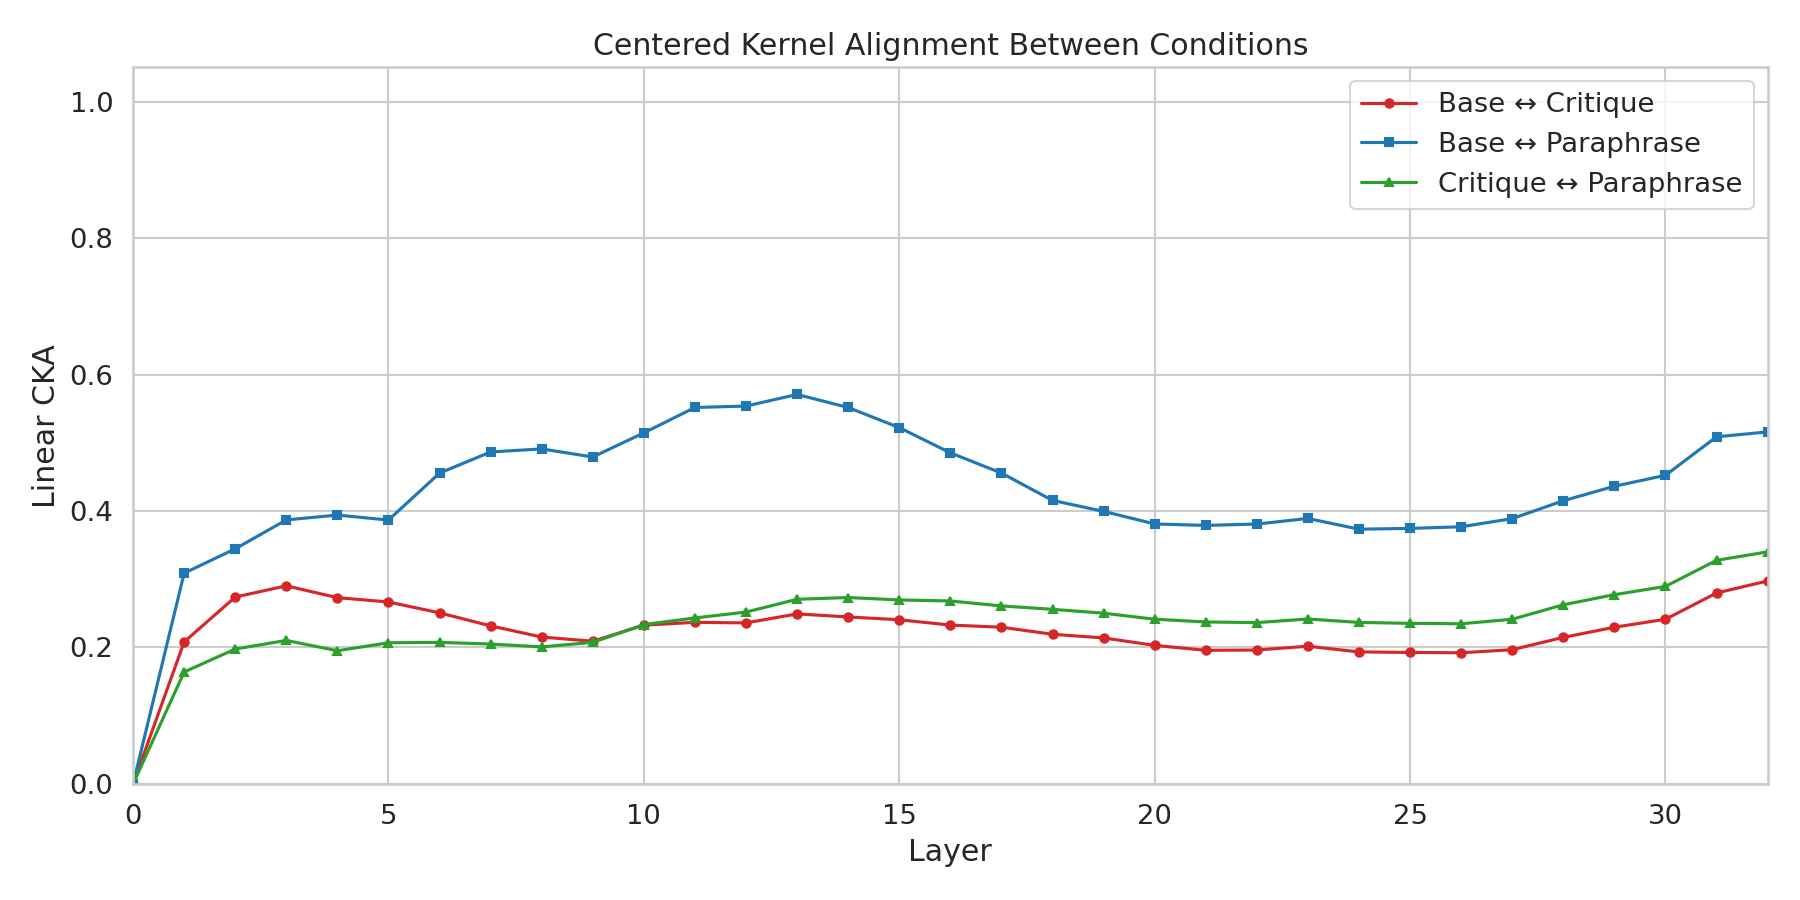
\includegraphics[width=\textwidth]{figures/cka_per_layer.png}
        \caption{CKA across layers}
        \label{fig:cka}
    \end{subfigure}
    \hfill
    \begin{subfigure}[b]{0.48\textwidth}
        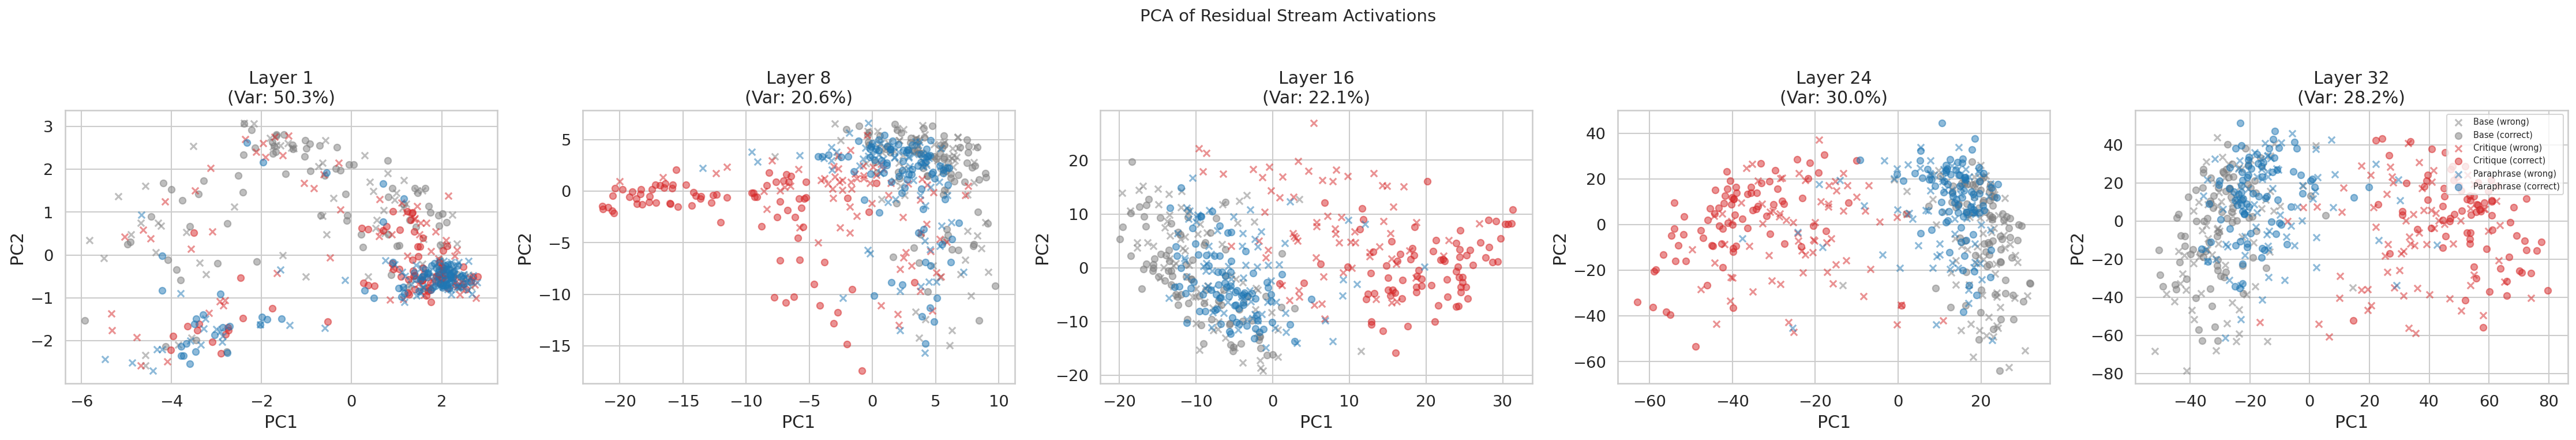
\includegraphics[width=\textwidth]{figures/pca_visualization.png}
        \caption{PCA visualization}
        \label{fig:pca}
    \end{subfigure}
    \caption{\captiona Per-layer CKA between conditions. Base$\leftrightarrow$paraphrase CKA is consistently higher than base$\leftrightarrow$critique, confirming that critique produces more divergent representational structure. \captionb PCA projection of activations at a representative later layer, showing clear separation between conditions.}
    \label{fig:cka_pca}
\end{figure}

\subsection{Linear Probe Accuracy: A Cautionary Finding}

\begin{table}[t]
    \centering
    \caption{Linear probe accuracy for classifying correct vs.\ incorrect initial answers. Evaluated via 5-fold stratified cross-validation. Majority-class baseline is 0.533 (80 correct, 70 incorrect). The high critique accuracy is largely driven by explicit correctness information in critique text (see \secref{sec:discussion}).}
    \begin{tabular}{@{}lcc@{}}
        \toprule
        Condition & Best Accuracy & Best Layer \\
        \midrule
        Base & 0.587 {\scriptsize $\pm$ 0.058} & 32 \\
        Paraphrase & 0.687 {\scriptsize $\pm$ 0.065} & 30 \\
        Critique & \textbf{0.973} {\scriptsize $\pm$ 0.039} & 17 \\
        \bottomrule
    \end{tabular}
    \label{tab:probe}
\end{table}

\Tabref{tab:probe} shows that linear probes achieve 97.3\% accuracy on critique activations compared to 58.7\% on base activations. However, this result requires careful interpretation: critique text explicitly states whether errors exist (\eg ``the answer is correct'' or ``there is an error in step 2''), so the high probe accuracy largely reflects the model encoding this explicit textual information rather than an emergent correctness representation. The paraphrase condition (68.7\%) provides a more informative middle ground---it slightly improves over base despite containing no evaluative content, suggesting that additional text context alone provides modest separability gains.

\subsection{Summary of Hypothesis Tests}

\begin{table}[t]
    \centering
    \caption{Summary of hypothesis testing results. All four hypotheses receive at least partial support from the data.}
    \begin{tabular}{@{}p{5.5cm}cc@{}}
        \toprule
        Hypothesis & Supported? & Key Evidence \\
        \midrule
        H1: Critique $>$ paraphrase drift & Yes & $\Delta$cos = 0.041, $p < 10^{-14}$ \\
        H2: Improved linear separability & Yes$^*$ & 97.3\% vs.\ 58.7\% \\
        H3: Layer-specific concentration & Partial & Peak at layers 12--16 \\
        H4: Consistent drift direction & Yes & 0.596 vs.\ 0.479 \\
        \bottomrule
    \end{tabular}
    \begin{flushleft}
    {\scriptsize $^*$Confounded by explicit correctness information in critique text; see \secref{sec:discussion}.}
    \end{flushleft}
    \label{tab:hypotheses}
\end{table}
